\documentclass[a4paper,12pt]{article}

\usepackage{amsmath}
\usepackage{amssymb}
\usepackage{color}
\usepackage{graphicx}
\usepackage{float}
\usepackage{listings}
\usepackage{lmodern}
\usepackage{mdframed}
\usepackage{url}
\usepackage{tikz}
\usetikzlibrary{shapes,arrows,positioning}
\usepackage{booktabs}
\usepackage{multirow}

\newcommand{\BlackBox}{\rule{1.5ex}{1.5ex}}

\definecolor{blue}{rgb}{0,0,0.8}
\definecolor{dkgreen}{rgb}{0,0.6,0}
\definecolor{gray}{rgb}{0.5,0.5,0.5}
\definecolor{mauve}{rgb}{0.58,0,0.82}

\lstset
{
   basicstyle=\ttfamily\footnotesize,
   language=C++,
   numbers=right,
   numberstyle=\color{gray},
   showtabs=true,
   breaklines=true,
   breakatwhitespace=true,
   captionpos=bottom,
   keywordstyle=\color{blue},
   commentstyle=\color{dkgreen},
   stringstyle=\color{mauve},
   frame=single
}

\mdfsetup
{
   skipabove=\topskip,
   skipbelow=\topskip,
   leftmargin=2em,
   rightmargin=2em
}


\title
{
   \includegraphics[width=12cm]{up-logo.jpg} \\
   \vspace{2cm}
   \textbf{COS700 Research Report} \\ \vspace{0.5cm}
   \textbf{Comparative analysis of Genetic Programming, Reinforcement Learning, and A* for Training Snake Game-Playing Agents} \\ \vspace{0.5cm}
   \textbf{Student number:} u20477181 \\ \vspace{0.5cm}
   \textbf{Supervisor(s)}: \\ Mr W Van Heerden
}

\author{Ennis Maphasha}

\date{July 2025}

\begin{document}

\maketitle

\newpage
\linespread{1.241}

\section*{Abstract}
This research provides a comparative analysis of three distinct approaches to train intelligent agents for playing the Snake game: 
Genetic Programming (GP), Deep Q-Learning (a Reinforcement Learning technique), 
and the A* search algorithm. 
The Snake game represents a classic environment where an agent must navigate a snake avatar through a two-dimensional grid to collect food while avoiding collisions with walls and its growing body. 

Genetic Programming employs evolutionary principles to evolve tree-based strategies through generations of candidate solutions, 
selecting and refining those that perform best according to a fitness function. 
Reinforcement Learning, specifically Deep Q-Learning, uses neural networks to learn optimal actions through experience and reward mechanisms. 
A* represents a deterministic pathfinding algorithm that can calculate optimal routes between the snake and food based on heuristic evaluations.

The research will be tested through a series of experiments where agents trained using each approach will play the Snake game under identical conditions. 
Performance metrics will include average score (food items collected), survival time, and strategy interpretability.

The novel contribution of this research lies in its comprehensive comparison of these three distinct paradigms within a single well-defined problem space, 
with particular emphasis on the viability of Genetic Programming as an alternative to the more commonly used Deep Reinforcement Learning techniques. 

The study aims to identify specific scenarios and conditions under which each approach excels, 
providing insights into the trade-offs between computational efficiency, performance, and strategy interpretability. 
The objective is to expand the toolkit for game-playing AI development, particularly where adaptability and solution transparency are prioritized over raw performance.

\section*{Keywords:}
Artificial Intelligence, Genetic Algorithm, Genetic Programming, Snake Game, Reinforcement Learning, Game AI

\newpage

\section{Introduction}
Games in research have provided a complex challenge for Artificial Intelligence (AI) systems to overcome while providing a platform for creative expression~\cite{Aiforgames}.
This combination lets games provide the unique advantage of a mix of scientific problem-solving and artistic creativity, making games extremely important to AI research.
This creates a mutually beneficial relationship where AI scientific research benefits from the complexity that games provide.
In return, the gaming industry has experienced significant evolution through AI technologies such as AI for Non-Playable Character (NPC) behavior, Procedural Level Generation and Player Experience Modeling \cite{AiInGames}.
This creates a cycle where progress in one field contributes to innovation in the other field \cite{Aiforgames}.

Artificial intelligence has been successfully applied to a variety of games like Tron \cite{tron}, Chess \cite{chess} and Atari games~\cite{atari}. 
In the context of AI and games, an \textit{agent} refers to an autonomous computational entity that perceives its environment through sensors, processes this information using decision-making algorithms, and takes actions to achieve specific objectives or maximize performance metrics \cite{AImodern}. 
Game-playing agents are AI systems specifically designed to interact with game environments, learning strategies and making decisions to achieve game-specific goals such as maximizing score, minimizing completion time, or surviving as long as possible.

When developing AI agents for games, the game environment provides a structured framework with clearly defined rules, objectives, and constraints. 
These rules serve multiple purposes: they define the legal actions available to the agent, establish the consequences of different actions, and specify the criteria for success or failure. 
The agent's role is to learn how to navigate these rules effectively, developing strategies that lead to optimal or near-optimal performance. 
This learning process can occur through various approaches, including reinforcement learning where agents learn through trial and error, supervised learning where agents learn from expert demonstrations, or evolutionary approaches where successful strategies emerge through iterative improvement across generations of candidate solutions.

The training process for game-playing agents typically involves exposing the agent to numerous game scenarios, allowing it to explore different actions and observe their outcomes. 
Through this experience, the agent develops an understanding of which actions lead to favorable results and which should be avoided. 
The agent's decision-making process evolves from random or rule-based actions toward sophisticated strategies that can adapt to changing game conditions and opponent behaviors.~\cite{AImodern}

The game of Snake consists of three ``entities" in the environment: the snake, the food, and the boundaries. 
There are three main rules to consider: When the snake "eats" the food, the tail grows by one unit, and the games score increases by one. 
If the snake runs into the boundaries, the snake "dies" and the game ends. If the snake runs into itself, the snake "dies" and the game ends. 
The goal of the game is to eat as much food as possible without the snake running into the boundaries or itself. 
The game is played on a two-dimensional grid, and the snake can move in 4 directions: up, down, left, and right. 
The snake can only move one unit at a time. The snake eats food as it moves over a food item.

Genetic Programming (GP) is a type of evolutionary algorithm that makes use of the principles of natural selection and reproduction
to evolve functions or programs that can be used to solve problems \cite{Koza}. In a Genetic program, a population of individual programs
consist of functions and terminals which are iteratively improved and evolved over generations through the use of genetic operators such as
crossover, mutation and reproduction. A fitness function is used to evaluate and quantify the performance of each individual on the target task.
The most successful, or ``fittest" individuals are selected to reproduce and generate the next generation of programs\cite{GPTut}

For problem domains where explicit programming is difficult or infeasible, GP has been used for automatic problem synthesis and machine learning,
The use of GP for has become prominent for evolving solutions that can adapt to complex and changing environments and has been used for applications
such as: bioinformatics \cite{Bioinformatics} and finance \cite{finance}.


This research proposes a novel approach of using genetic programming to train agents to play the game of Snake. 
Other methods of training Snake game playing agents make use of primarily Reinforcement Learning (RL) \cite{Reinforcement1} and deep learning \cite{Reinforcement4} and the use of heuristic path-finding approaches \cite{Heuristic1} and genetic algorithms \cite{EA2}, 
which successfully train agents to play Snake, but are not effective at training agents that will reach the end of the game.

\section{Problem Statement (must expand)}
\textbf{Can GP produce competitive AI agents for the Snake game compared to traditional RL methods?}

Due to a lack of similar GP based methods applied to Snake, GPs potential to evolve interpretable, adaptive strategies remains less explored than similar dominant strategies. 
This research aims to address this gap by designing a framework for Snake, 
evaluating its performance against Reinforcement learning (RL) baselines. 
The project aims to determine if GP can complement or compete with RL.

This research aims to:
\begin{itemize}
   \item Determine whether GP can train Snake agents that can compete with, 
   or outperform traditional game-playing agents in terms of score and survival time. This will be addressed by the following steps:
   \begin{itemize}
      \item Develop a Genetic Programming framework for the Snake game environment.
      \item Compare GP agents with traditional RL and rule-based agents using performance metrics like average score, survival time and computational cost.
      \item Identify limitations and challenges of GP and propose potential solutions.
      \item Investigate the interpretability of GP agents and their ability to adapt to different game scenarios.
   \end{itemize}
\end{itemize}

This research does not consider: 
\begin{itemize}
   \item Generalizing findings to other games in similar domains.
   \item Other computational intelligence approaches such as Particle swarm optimization.
\end{itemize}

\section{Methodology}

This research adopts an empirical experimental approach to investigate the effectiveness of genetic programming (GP) for training Snake game agents compared to traditional baseline methods. The methodology involves implementing and evaluating three distinct approaches: A* pathfinding as a deterministic baseline, Deep Q-Network (DQN) as a reinforcement learning baseline, and genetic programming as the primary investigation focus.

\subsection{Experimental Framework}

The framework utilizes a standardized Snake game environment to ensure fair comparison across all three approaches. The Snake game implementation features a configurable grid-based environment where agents must navigate a snake avatar to collect food while avoiding collisions with walls and the snake's own body. The environment provides consistent state representation and reward mechanisms across all agent implementations.

\subsubsection{State Representation}

The game state is represented through an 11-dimensional feature vector that captures essential environmental information while maintaining computational efficiency. This unified state representation enables direct comparison between different algorithmic approaches while providing sufficient complexity for meaningful agent evaluation. The feature vector design prioritizes local awareness over global state information, reflecting the constraint that agents should make decisions based on immediately relevant environmental factors.

The 11-dimensional state vector $\mathbf{s} = [s_0, s_1, \ldots, s_{10}]$ is constructed as illustrated in Figure~\ref{tab:state_vector_components}, where each component encodes specific environmental information:

% state vector png
\begin{figure}[H]
   \centering
   \includegraphics[width=0.6\textwidth]{vector_analysis.png}
   \caption{11-Dimensional State Vector Representation}
   \label{fig:state_vector}
\end{figure}

\begin{table}[H]
         \begin{tabular}{|c|c|c|}
      \hline
      \textbf{Index} & \textbf{Component} & \textbf{Value} \\
      \hline
      0 & Danger Up & 1.0 \\
      1 & Danger Right & 0.0 \\
      2 & Danger Down & 0.0 \\
      3 & Danger Left & 1.0 \\
      4 & Direction UP & 0.0 \\
      5 & Direction RIGHT & 1.0 \\
      6 & Direction DOWN & 0.0 \\
      7 & Direction LEFT & 0.0 \\
      8 & Food X-direction & -1.0 \\
      9 & Food Y-direction & 1.0 \\
      10 & Snake Length & 0.12 \\
      \hline
      
      \end{tabular}
      \caption{State vector components}
      \label{tab:state_vector_components}
\end{table}


\textbf{Danger Detection (Components 0-3):} These binary indicators detect immediate collision threats in the four cardinal directions relative to the snake's head position. A value of 1.0 indicates that moving in the corresponding direction would result in collision with either the environment boundary or the snake's own body, while 0.0 indicates a safe movement option. This local danger awareness enables agents to avoid immediate fatal actions without requiring global environment knowledge.

\textbf{Current Direction Encoding (Components 4-7):} The snake's current movement direction is encoded using one-hot representation, where exactly one component has value 1.0 and the others are 0.0. This encoding prevents agents from selecting actions that would cause the snake to immediately reverse direction, which constitutes an invalid move in the Snake game mechanics.

\textbf{Food Direction Indicators (Components 8-9):} These components encode the relative position of food with respect to the snake's head using signed values. Component 8 represents horizontal food direction: +1.0 if food is to the right, -1.0 if to the left, and 0.0 if directly aligned. Component 9 represents vertical food direction: +1.0 if food is below, -1.0 if above, and 0.0 if aligned. This encoding provides agents with goal-oriented information to guide movement towards rewards.

\textbf{Snake Length Normalization (Component 10):} The final component represents the current snake length normalized by the maximum possible length (grid width × height). This value starts near 0.0 for a short snake and approaches 1.0 as the snake grows, providing agents with progress information and enabling length-aware decision-making.

\subsection{Baseline Implementation}

The experimental framework employs two baseline algorithms to provide performance benchmarks for comparison with the genetic programming approach. These baselines represent established methodologies from different algorithmic paradigms: deterministic pathfinding and reinforcement learning.

\subsubsection{A* Pathfinding Algorithm}

The A* pathfinding algorithm serves as the deterministic baseline for this study, providing an optimal solution approach under perfect information conditions. A* combines the advantages of Dijkstra's algorithm's guarantee of finding the shortest path with the efficiency of greedy best-first search through the use of an admissible heuristic function.

\paragraph{Algorithm Fundamentals}

The A* algorithm maintains a priority queue of candidate paths, where each path is evaluated using the cost function:

\begin{equation}
f(n) = g(n) + h(n)
\end{equation}

Where $g(n)$ represents the actual cost from the start position to node $n$, and $h(n)$ is the heuristic estimate of the cost from node $n$ to the goal. For the Snake game implementation, the Manhattan distance serves as the heuristic function:

\begin{equation}
h(n) = |x_n - x_{goal}| + |y_n - y_{goal}|
\end{equation}

This heuristic is admissible for grid-based movement since it never overestimates the actual distance to the goal, ensuring the optimality of the A* solution.

Unlike traditional pathfinding problems with static obstacles, the snake's body is a dynamic obstacle that changes after each move. The implementation accounts for this temporal aspect by allowing the tail cell to be considered safe when the snake is not expected to grow. This logic treats the tail differently depending on whether the planned path will consume food (i.e., increase snake length).

The algorithm uses a two-part collision check:
\begin{itemize}
   \item \textbf{Immediate Collision Detection:} Validate candidate neighbor cells against walls and the snake's current body positions.
   \item \textbf{Future State Validation:} When evaluating moves during search, the algorithm factors whether the snake would grow (eat food) along the planned path; if it would not grow, the current tail is treated as vacated and may be used by the path.
\end{itemize}

	\textbf{Path Representation and Action Selection:} The A* search maintains a priority queue (open set) storing tuples with the f-cost (\(g+h\)), g-cost, the current position and the path taken so far. When a path to the food is found the algorithm returns the full ordered list of grid coordinates from head to food. The agent selects the immediate action by comparing the snake head with the next coordinate in that returned path and mapping the position difference to a directional command (UP, DOWN, LEFT, RIGHT).

\paragraph{Fallback Mechanisms}

When no direct path to food exists, the A* agent employs fallback strategies to maintain game survival:

	\textbf{Space Accessibility Analysis:} To choose among survival moves the agent simulates each valid immediate action by making a copy of the game state and applying the candidate action. From the resulting head position the agent performs a breadth-first search to count how many grid cells are reachable while treating the (simulated) snake body as obstacles. This reachable cell count is used as an accessibility score that estimates how safe a move is with respect to becoming trapped.

	\textbf{Safe Move Selection:} For each candidate move the implementation records the accessibility score and the immediate reward observed during the simulated step. Candidate moves are ranked primarily by accessibility (larger is better) and secondarily by immediate reward; the selected move maximizes survival area first and prize-seeking behavior second. If no safe moves are found the agent falls back to any valid action reported by the environment.

\subsubsection{Deep Q-Learning Implementation}

The Deep Q-Learning (DQN) baseline represents the reinforcement learning approach. It uses the same 11-dimensional feature vector (Section~\ref{tab:state_vector_components}), enabling a fair, like-for-like comparison with A* and GP.

\paragraph{Markov Decision Process Formulation} We model Snake as an MDP $(\mathcal{S},\mathcal{A},P,r,\gamma)$ with:
\begin{itemize}
   \item State $s\in\mathcal{S}$: the 11-D vector encoding danger, current heading, food direction, and normalized length.
   \item Actions $a\in\mathcal{A}=\{\textsc{Up},\textsc{Down},\textsc{Left},\textsc{Right}\}$.
   \item Transition $P(s'\mid s,a)$: induced by the Snake dynamics.
   \item Reward $r(s,a,s')$: positive for eating food, negative for collisions, and a small step cost to encourage efficiency.
   \item Discount $\gamma\in(0,1)$: balances immediate reward and long-term survival.
\end{itemize}

\paragraph{Network and Targets} A feed-forward Q-network $Q_\theta(s,a)$ maps the 11-D state to 4 action-values. We use a Multi-layer Perceptron (MLP) with hidden sizes [128, 128, 64] and ReLU activations, optimized with Adaptive moment estimation (Adam). A separate target network $Q_{\theta^-}$ is updated periodically to stabilize training. The Bellman target and loss are:
\begin{equation}
   y = r + \gamma\,(1-\mathbb{1}_{\text{done}})\max_{a'} Q_{\theta^-}(s',a'),
\end{equation}
\begin{equation}
   \mathcal{L}(\theta) = \big(Q_\theta(s,a) - y\big)^2.
\end{equation}

\paragraph{Sample Efficiency and Stability} The agent employs:
\begin{itemize}
   \item Experience replay: a finite buffer storing tuples $(s,a,r,s',\text{done})$; training samples uniformly from this buffer (mini-batches).
   \item Target network updates: copy $\theta\to\theta^-$ every $K$ updates to reduce moving-target instability.
   \item $\epsilon$-greedy exploration: start with high exploration and decay $\epsilon$ towards a small floor to favour exploitation.
   \item Gradient clipping: to prevent exploding gradients during unstable phases.
\end{itemize}

\paragraph{Reward Design} The reward follows the environment: strong positive for food consumption, strong negative for collisions (wall or body), and a small living penalty to promote shorter, purposeful paths. This shaping aligns the agent towards survival while maintaining pressure to reach food efficiently.

\paragraph{Training Protocol} For each episode: initialize the environment, then iterate until termination or a step cap:
\begin{enumerate}
   \item Select action with $\epsilon$-greedy from $Q_\theta(s,\cdot)$.
   \item Step the environment to obtain $(r,s',\text{done})$; store $(s,a,r,s',\text{done})$ in replay memory.
   \item If memory $\ge$ batch size, sample a mini-batch and perform a gradient step on $\mathcal{L}(\theta)$.
   \item Every $K$ optimization steps, update the target network parameters $\theta^-\leftarrow\theta$.
   \item Decay $\epsilon$ after each episode.
\end{enumerate}

\subsection{Genetic Programming Implementation}

The genetic programming approach represents the primary focus of this research, evolving tree-based decision policies that map the 11-dimensional state vector to directional actions. Unlike the deterministic A* approach or the neural network-based DQN method, GP evolves interpretable symbolic programs that can be directly analyzed and understood.

\subsubsection{Tree Representation}

The GP implementation uses a binary tree representation where each individual in the population represents a complete decision policy for the Snake game. The tree structure consists of two fundamental node types:

\paragraph{Action Nodes (Terminal Nodes)} These leaf nodes represent the four possible movement actions: UP, DOWN, LEFT, and RIGHT. When evaluated, an action node returns its corresponding Direction value directly. Action nodes serve as the terminal elements of the decision tree and represent the final output of the policy evaluation process.

\paragraph{Condition Nodes (Internal Nodes)} These internal nodes implement conditional logic based on the state vector features. Each condition node contains four key components:
\begin{itemize}
   \item \textbf{Feature Index:} An integer (0-10) specifying which component of the state vector to examine
   \item \textbf{Threshold Value:} A floating-point threshold for comparison
   \item \textbf{Left Child:} The subtree executed when the condition evaluates to true (feature value \textgreater~threshold)
   \item \textbf{Right Child:} The subtree executed when the condition evaluates to false (feature value $\le$ threshold)
\end{itemize}

The tree evaluation process follows a standard recursive descent pattern where condition nodes compare their assigned state vector component against their threshold value, then delegate evaluation to the appropriate child subtree.

\subsubsection{Population Initialization}

The initial population generation aims to balance tree diversity with domain-specific knowledge. The random tree generation process incorporates several key features:

\paragraph{Feature Selection} Rather than selecting state vector features uniformly at random, the initialization process biases towards more meaningful features. Danger detection features (indices 0-3) and food direction features (indices 8-9) are selected with 70\% probability, while other features are chosen with 30\% probability. This bias reflects the importance of collision avoidance and goal-seeking behavior in the Snake domain.

\paragraph{Threshold Selection} Threshold values are generated based on the semantic meaning of each feature type:
\begin{itemize}
   \item \textbf{Danger Features (0-3):} Fixed threshold of 0.5 for binary danger indicators
   \item \textbf{Direction Features (4-7):} Fixed threshold of 0.5 for one-hot direction encoding
   \item \textbf{Food Direction Features (8-9):} Random threshold in range [-0.5, 0.5] for signed directional values
   \item \textbf{Snake Length Feature (10):} Random threshold in range [0.1, 0.9] for normalized length values
\end{itemize}

\paragraph{Depth Control Mechanisms} The tree generation process implements both hard and soft depth limits. Trees are prevented from exceeding a maximum depth, while a probabilistic early termination mechanism (40\% probability) promotes the creation of smaller, more manageable trees during initialization.

\subsubsection{Genetic Operators}

\paragraph{Crossover Operation} The crossover operator implements subtree exchange between two parent trees. The process involves:
\begin{enumerate}
   \item Creating deep copies of both parent trees to preserve the original population
   \item Identifying all condition nodes (internal nodes) in both trees as potential crossover points
   \item Randomly selecting one condition node from each parent tree
   \item Swapping the complete subtrees rooted at the selected nodes
\end{enumerate}

This approach ensures that crossover operations maintain valid tree structures while allowing meaningful exchange of decision-making logic between high-performing individuals.

\paragraph{Mutation Operation} The mutation operator employs a recursive replacement strategy with configurable mutation rates. When a node is selected for mutation, it is replaced entirely with a newly generated random subtree of appropriate depth. This replacement-based approach ensures that mutations can introduce significant structural changes while maintaining tree validity.

The mutation process traverses the tree recursively, applying mutation probability at each node independently. For condition nodes, mutation can be applied to the node itself or propagated to its children, allowing for both local and global structural modifications.

\subsubsection{Fitness Evaluation}

The fitness function implements a multi-objective evaluation strategy that balances multiple performance criteria across multiple game episodes. For each individual tree, fitness is calculated as the average performance over 5 independent game episodes on a 12×12 grid environment.

\paragraph{Fitness Components} The fitness function combines three weighted components:
\begin{equation}
   \text{Fitness} = \text{food\_collected} \times 2000 + \text{steps\_survived} \times 1 + \text{food\_bonus}
\end{equation}

Where the food bonus equals 100 if any food was collected during the episode, and 0 otherwise. This weighting scheme heavily prioritizes food collection while providing secondary rewards for survival time and basic competency.

\paragraph{Episode Management} Each fitness evaluation runs the tree policy through complete game episodes, tracking both immediate rewards and survival duration. The state vector is updated after each action, ensuring that the tree policy operates on current environmental information throughout the episode.

\subsubsection{Selection and Population Management}

\paragraph{Tournament Selection} The selection mechanism employs tournament selection with a tournament size of 5 individuals. For each selection event, 5 individuals are randomly chosen from the population, and the individual with the highest fitness value wins the tournament. This approach maintains selection pressure towards high-performing individuals while preserving diversity through the random tournament composition.

\paragraph{Elitism Strategy} The implementation incorporates elitism by preserving the top 50 individuals in each generation. These elite individuals are carried forward unchanged to the next generation, ensuring that high-quality solutions are not lost due to genetic operations.

\paragraph{Diversity Maintenance} To combat genetic diversity loss and population stagnation, the algorithm monitors fitness improvement over generations. When no improvement is observed for 50 consecutive generations, a diversity injection mechanism replaces the bottom 20\% of the population with newly generated random individuals.

\paragraph{Stagnation Detection} The algorithm tracks the number of consecutive generations without fitness improvement. This stagnation counter triggers diversity injection, providing a feedback mechanism for population health monitoring.

\subsubsection{Algorithm Parameters}

The GP implementation uses the following default parameters, optimized through preliminary experimentation:
\begin{itemize}
   \item \textbf{Population Size:} 130 individuals
   \item \textbf{Generations:} 5000 maximum iterations
   \item \textbf{Maximum Tree Depth:} 4–5 levels
   \item \textbf{Base Mutation Rate:} 0.3
   \item \textbf{Crossover Rate:} 0.7
   \item \textbf{Elite Size:} 50 individuals
   \item \textbf{Diversity Threshold:} 50 generations
   \item \textbf{Tournament Size:} 5 individuals
\end{itemize}

These parameters represent a balance between exploration and exploitation, computational efficiency, and solution quality based on the specific characteristics of the Snake game domain.

\section{Background}

\subsection{Evolutionary Computation}
Evolutionary computation is a set of algorithms inspired by biological evolution and natural selection~\cite{Koza}. 
The basic idea comes from Charles Darwin's theory of evolution, where species adapt and improve over generations through 
selection, reproduction, and variation. In computing, this means maintaining populations of candidate solutions that are 
improved over time by selecting the best individuals, combining their successful features, and introducing new variations 
through mutation~\cite{GPTut}.

Evolutionary computation includes various bio-inspired techniques that work well for solving complex problems where traditional 
methods struggle. These approaches are particularly good for problems with large search spaces, multiple goals, or where the 
problem structure is not well understood. Evolutionary approaches work well because they can explore solution spaces broadly 
while focusing on promising areas, making them robust against getting stuck in local optima that trap other optimization methods.~\cite{EAs}

\subsection{Representation and Search Space}
Before exploring specific evolutionary algorithms, it is important to understand two fundamental concepts: representation and search space. 
These concepts form the foundation for how evolutionary algorithms encode, manipulate, and explore potential solutions.

\subsubsection{Representation}
Representation refers to how candidate solutions are encoded or structured within the evolutionary algorithm. 
This encoding determines how solutions are stored, manipulated, and evolved throughout the optimization process. 
The choice of representation is crucial because it directly affects what solutions can be discovered and how efficiently the algorithm can find them.

Common representation schemes include:
\begin{itemize}
   \item \textbf{Binary strings:} Solutions encoded as sequences of 0s and 1s, commonly used in genetic algorithms for parameter optimization
   \item \textbf{Real-valued vectors:} Solutions represented as arrays of real numbers, suitable for continuous optimization problems
   \item \textbf{Tree structures:} Hierarchical representations where solutions are encoded as trees, extensively used in genetic programming
   \item \textbf{Permutations:} Ordered sequences representing solutions to combinatorial problems like scheduling or routing
   \item \textbf{Variable-length structures:} Representations that allow solutions of different sizes, enabling structural evolution
\end{itemize}

The representation must be carefully designed to capture the essential features of the problem while allowing meaningful genetic operations. 
A good representation should be able to express all possible solutions, allow smooth transitions between similar solutions, 
and support effective genetic operations.~\cite{ECintro}

\subsubsection{Search Space}
The search space, also known as the solution space, encompasses all possible solutions that can be represented using the chosen encoding scheme. 
This space defines the boundaries within which the evolutionary algorithm operates and determines the scope of solutions that can potentially be discovered.~\cite{ECintro}

\subsection{Evolutionary Algorithms}
Evolutionary algorithms form a subset of evolutionary computation techniques that specifically use mechanisms inspired by biological evolution 
to iteratively explore and exploit solutions to real world problems. The major components of evolutionary algorithms can be represented 
by the cyclical process shown in Figure~\ref{fig:ea_process}, which includes:

\begin{figure}[H]
\centering
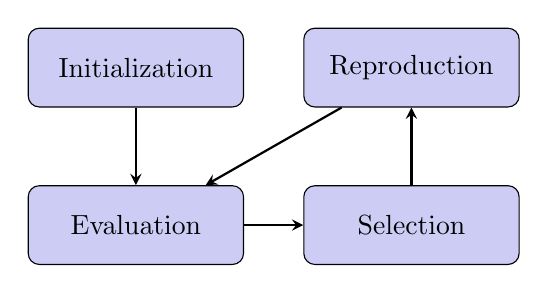
\begin{tikzpicture}[node distance=2cm,
    box/.style={rectangle, draw, fill=blue!20, text width=2.5cm, text centered, rounded corners, minimum height=1cm},
    decision/.style={diamond, draw, fill=yellow!20, text width=2cm, text centered, aspect=2},
    arrow/.style={thick,->,>=stealth}]
    
    % Nodes
    \node [box] (init) {Initialization};
    \node [box, below of=init] (eval) {Evaluation};
    \node [box, right of=eval, node distance=3.5cm] (select) {Selection};
    \node [box, above of=select] (reprod) {Reproduction};
    
    % Arrows
    \draw [arrow] (init) -- (eval);
    \draw [arrow] (eval) -- (select);
    \draw [arrow] (select) -- (reprod);
    \draw [arrow] (reprod) -- (eval);
    
\end{tikzpicture}
\caption{Evolutionary Algorithm Process Flow}
\label{fig:ea_process}
\end{figure}

\subsubsection{The evolutionary process}
The evolutionary algorithm process shown in Figure~\ref{fig:ea_process} consists of four main components which can be further elaborated as follows:

\begin{enumerate}
   \item During \textbf{Initialization}, a random population of candidate solutions is generated using a representation that best matches the problem domain. 
   These candidate solutions represent potential solutions to the problem. 
   Each represents a point in the search space.
   \item Each candidate solution passes through the \textbf{Evaluation} phase, where the viability of a solution to solve the problem is assessed. 
   This viability is quantified using a fitness function.
   The fitness function represents a measure of how well a candidate solution performs the desired task. 
   The function is problem specific and drives the evolutionary process by either rewarding or penalizing solutions based on the solutions' ability to meet the problem objectives.
   \item Once each candidate solution has been evaluated and assigned some fitness measure, the \textbf{Selection} phase is used to select individuals for reproduction. 
   Selection is used propagate higher quality individuals from one generation to the next, which,
   for some problem domains, allows high quality traits to be combined and refined across generations. 
   This process allows for the controlled exploration and exploitation of the solution space. 
   This exploration of the search space allows for diversity in the potential areas of the search space being evaluated.
   Exploitation helps guide the search to more promising areas of the search space.~\cite{EAs}
   \item After viable individuals are selected, the \textbf{Reproduction} phase uses genetic operators to create new candidate solutions from the viable individuals selected in the previous phase.
   Common genetic operators include: \textbf{Crossover}, which involves an exchange of genetic material between two parent solutions to create offspring that inherit characteristics from both parents.~\cite{EAs}
   \textbf{Mutation}, which introduces random changes to a candidate solution, producing a new unique solution that represents a new point in the search space.~\cite{EAs} 
\end{enumerate}

\subsection{Genetic Algorithms}
Genetic Algorithms (GAs) are a specific type of evolutionary algorithm that use principles inspired by natural genetics and Darwin's theory of evolution to solve optimization and search problems~\cite{EAs}.
GAs have become one of the most widely used evolutionary computation techniques due to their simplicity, robustness, and effectiveness across diverse problem domains~\cite{ECR}.

\subsubsection{Core Components of Genetic Algorithms}
A genetic algorithm operates on a population of candidate solutions, where each solution is typically represented as a fixed-length string of symbols, commonly binary strings. The algorithm follows the general evolutionary process described earlier, but with specific implementations of each component:

\textbf{Representation:} In traditional GAs, solutions are encoded as chromosomes, 
typically represented as binary strings where each bit position corresponds to a specific parameter or decision variable. 

\textbf{Fitness Function:} The fitness function evaluates how well each chromosome solves the target problem. 
This function assigns a numerical fitness value to each individual, which directly influences their probability of being selected for reproduction. 
The design of an appropriate fitness function is crucial for the success of the GA~\cite{EAs}.

\textbf{Selection Methods:} GAs employ various selection strategies to choose parents for reproduction. Common methods include:
\begin{itemize}
   \item \textbf{Tournament Selection:} Randomly selects a subset of individuals and chooses the fittest among them
   \item \textbf{Roulette Wheel Selection:} Assigns selection probability proportional to fitness values
   \item \textbf{Rank-based Selection:} Selects individuals based on their fitness rank rather than absolute fitness values
\end{itemize}

\textbf{Genetic Operators:} The primary operators in GAs are crossover and mutation:
\begin{itemize}
   \item \textbf{Crossover:} Combines genetic material from two parent chromosomes to create offspring.
   Common crossover methods include single-point, multi-point, and uniform crossover
   \item \textbf{Mutation:} Introduces random changes by flipping bits in binary representations, 
   helping maintain population diversity and preventing premature convergence
\end{itemize}

\subsection{Genetic Programming}
Genetic Programming (GP) extends the principles of genetic algorithms to evolve complete computer programs rather than fixed-length parameter strings~\cite{Koza}. 
GP represents a paradigm shift from optimizing parameters to evolving the structure and logic of programs themselves~\cite{GPTut}.

\subsubsection{Fundamental Concepts}
Unlike genetic algorithms that work with fixed-length chromosomes, genetic programming operates on variable-length tree structures that represent executable programs. 
These trees consist of:

\textbf{Function Set:} Internal nodes of the tree containing functions, operators, or control structures that can be executed. Examples include mathematical operators (+, -, *, /), logical operators (AND, OR, NOT), conditional statements (IF-THEN-ELSE), and domain-specific functions~\cite{GPP}.

\textbf{Terminal Set:} Leaf nodes representing variables, constants, or input values that serve as operands for the functions. These provide the basic building blocks from which more complex expressions can be constructed~\cite{GPTut}.

The combination of function and terminal sets defines the search space of possible programs that GP can evolve. The choice of these sets is crucial as they determine the expressiveness and complexity of solutions that can be discovered.

\subsubsection{Tree Representation and Genetic Operations}
GP uses tree-based representations where each individual program is encoded as a parse tree. This representation allows for natural implementation of genetic operations:

\textbf{Crossover in GP:} The most common crossover operation involves selecting random subtrees from two parent programs and exchanging them. This creates offspring that inherit different functional components from both parents, potentially combining successful sub-strategies~\cite{Koza}.

\textbf{Mutation in GP:} Mutation operations can involve:
\begin{itemize}
   \item \textbf{Point Mutation:} Randomly changing a function or terminal at a specific node
   \item \textbf{Subtree Mutation:} Replacing an entire subtree with a randomly generated new subtree
   \item \textbf{Hoist Mutation:} Replacing a subtree with one of its own subtrees, effectively simplifying the program
\end{itemize}

\textbf{Selection and Reproduction:} Similar to GAs, GP uses fitness-based selection to choose individuals for reproduction. 
The fitness function evaluates how well each program performs on the target task, such as game-playing performance or problem-solving accuracy~\cite{GPP}.

\subsection{Reinforcement Learning}
Reinforcement Learning (RL) focuses on the agents' ability to make decisions by actively interacting with their environment.
The agent learns to achieve a goal by taking actions and adjust based on positive or negative feedback in the form of punishments or rewards.
This means the agents can improve its strategy over time through trial and error. \cite{DRL}

In RL, a policy is used to describe how a learning agent behaves at a given time, a policy is used 
to map a state in the environment to actions that can be taken when in those states. \cite{ReinforcementIntro}

\subsubsection{Deep Reinforcement Learning}
Deep Q Reinforcement Learning (DQL) \cite{DQL} uses a deep neural network to find an optimal Q-value or action-value function.
The Q-value represents the expected future rewards when an agent starts at a given state and takes a specific action.
This state-action pair is used to determine the best action to take in a given state.
The Action-value function maps each state-action pair to its Q-value, the expected future reward. These help
guide the agent to make decisions that will maximize long-term rewards based on the Q-value.

\subsubsection{Markov Decision Process}
The theoretical foundation for reinforcement learning lies in Markov Decision Processes (MDPs), which provide a mathematical framework for modeling decision-making problems where outcomes are partly random and partly under the control of a decision maker~\cite{markov}.

A Markov Decision Process is formally defined as a tuple $(S, A, P, R, \gamma)$ where:
\begin{itemize}
\item $S$ is a finite set of states representing all possible situations the agent can encounter
\item $A$ is a finite set of actions available to the agent
\item $P: S \times A \times S \to [0,1]$ is the state transition probability function, where $P(s'|s,a)$ represents the probability of transitioning to state $s'$ when taking action $a$ in state $s$
\item $R: S \times A \to \mathbb{R}$ is the reward function, where $R(s,a)$ gives the immediate reward for taking action $a$ in state $s$
\item $\gamma \in [0,1]$ is the discount factor that determines the importance of future rewards relative to immediate rewards
\end{itemize}

The fundamental property of an MDP is the Markov property, which states that the future state depends only on the current state and action, not on the sequence of events that preceded it.

The discount factor $\gamma$ plays a crucial role in balancing immediate versus long-term rewards. A value close to 1 encourages the agent to consider long-term consequences, while a value closer to 0 focuses on immediate rewards. This is particularly important in the Snake game where the agent must balance the immediate goal of collecting food with the long-term goal of avoiding collisions that become increasingly likely as the snake grows longer.

\section{Related Work}
\subsection{Overview}
A number of studies for Snake game playing agents have explored the use of Evolutionary Computation \cite{EA2}, 
Heuristic Search algorithms \cite{Heuristic1}, \cite{Heuristic2}, 
Hamiltonian Cycles \cite{Heuristic3}, Reinforcement learning with SARSA for movement \cite{Reinforcement1}, 
Deep reinforcement learning \cite{Reinforcement2}, Deep Q learning \cite{Reinforcement4} \cite{Reinforcement6} and Particle Swarm Optimization (PSO) \cite{Unsupervised1}.

\subsection{Evolutionary Algorithms}
Evolutionary computation and Evolutionary algorithms are a subset of computational intelligence techniques inspired by natural selection.
They make use of principles that model evolutionary evolution such as selection to find well-performing solutions, mutation to introduce 
diversity by randomly changing solutions, and crossover to combine traits from two parents to create a distinct offspring. \cite{EA2}

The use of Evolutionary computation has been effective, primarily focusing on automated optimization \cite{EA2}.

Yeh \textit{et al.} \cite{EA2} proposed a neural network approach that uses Evolutionary computation to optimize movement rating functions,
which are mathematical functions used by the AI controller to decide the moving direction of the snake. 
This approach is limited to optimizing the weights of the movement rating functions and does not allow for the evolution of new strategies or behaviors.
The controllers were optimized for fixed food layouts, limiting their adaptability to dynamic environments.

\subsection{Path Finding Algorithms}
When considering heuristic pathfinding approaches, studies have been conducted to evaluate the performance of various algorithms in the Snake game.
Mim \textit{et al.} \cite{Heuristic3} examined the performance of uninformed searches.
Breadth first search (BFS)~\cite{BreadthFirstSearch}, Depth first search (DFS)~\cite{DepthFirstSearch},
and informed searches (A*~\cite{A}, Best-First Search~\cite{Best}, Hamiltonian Search~\cite{Ham}) were investigated, and their performance compared against human players.
While the approaches had varying success rates, the A* algorithm was the most successful due to its heuristic optimization.
Other algorithms were less successful due to inefficiency in dynamic environments, or suboptimal pathfinding.

Sharma \textit{et al.} \cite{Heuristic2} examined BFS~\cite{BreadthFirstSearch}, A*~\cite{A}, an
A* variation combined with a Breadth First Search algorithm to examine if a path leads to a dead end.
A random move baseline was also examined that selected the next move randomly and an almighty move baseline which moves the snake in a pre-defined pattern across the board, allowing for no possibility of failure.
The investigation found the average scores achievable for each algorithm and used a combined approach where each algorithm was used in a sequence, 
BFS was used to eat the first 4 fruit, A* for the next 4 fruit and almighty move for the final 62 fruit. This approach was used as a way to mitigate
the limitations of individual algorithms and improve overall performance.

While heuristic pathfinding approaches have shown success in the Snake game, these methods show limitations in adaptability and generalization 
to dynamic environments which is a critical aim of this research.


\subsection{Reinforcement Learning}
After considering path finding algorithms, the proposal now considers Reinforcement Learning (RL), 
which has had many successful applications in games with its ability to learn through trial and-error interactions with a dynamic environment \cite{DRL}.


RL has been widely used in the Snake game, with various approaches such as SARSA \cite{Reinforcement1} 
and Deep Q-learning \cite{Reinforcement2}\cite{Reinforcement7}.


When using SARSA, 
Almalki \textit{et al.} \cite{Reinforcement1} found the use of SARSA for on-policy learning and DQL for off-policy learning.
On-policy learning represents agents that build upon the policy they are currently following,
while off-policy learning represents agents that build on policies from various other sources, not just the current policy.
The use of both off-policy and on-policy learning allows the algorithm to better adapt to dynamic environments, while having improved stability, However, the study does not comprehensively evaluate the performance of the agents against other algorithms.

When considering the use of Deep Q-learning, Wei \textit{et al.} \cite{Reinforcement7} 
propose the use of a custom reward mechanism based on a distance reward, where the reward given 
to the agent is higher when the agent is closer to the target, 
a training gap where the agent is prevented from learning for a time after it eats a fruit,
and a timeout strategy, which is a way to punish an agent if it fails to eat a fruit over some time steps.
The algorithm was evaluated against a baseline model and human players. The baseline model used was a DQL model trained in the same manner as the proposed algorithm, but with the omission of the custom reward mechanism, and training gap. The results showed the proposed algorithm outperforms both the baseline model and human players.
However, the results showed low average scores, but high survival steps resulting in longer play time.

Hossain \textit{et al.} \cite{Reinforcement2} proposed a Deep Q-learning approach, using standard Snake game rules, but leveraged the use of the Monte Carlo Method \cite{MonteCarlo} where the agents observable environment determines the next action to take.
In this method the agent will play the game until the game ends, then the policy is updated based on the rewards observed.
The agent will use the feedback given at the end of the game to evaluate how well previous states and actions performed.
Over time the algorithm was able to achieve a high average score, however, the algorithm was not evaluated against any other algorithms.
The approach taken is flawed in its use of manual Rewards systems where the actions taken by the snake have specific rewards associated 
e.g. ``Eat food +10, Game over -1" as it does not allow the agent to learn and adjust its priorities over time. The study also noted long term survivability issues
due to the agent colliding with itself since there is no global view of the environment.

When analyzing the use of Reinforcement learning and Deep Q-Learning, the algorithms can successfully learn to play Snake, however, the controllers have a dependency on the award systems used, therefore any miscalculations made in
the awards system lead to suboptimal performance. The algorithms also struggle with long-term survivability \cite{Reinforcement2} \cite{Reinforcement6} where the snakes will eventually collide with themselves.

\subsection{Unsupervised Learning}
Particle swarm optimization (PSO) \cite{PSOs} is a population-based optimization algorithm that is inspired by the social behavior of bird flocks.
The swarm is made up of particles, each particle represents a solution in the solution space.
The algorithm moves the particles through the solution space to find an optimal solution.

Van Heerden \textit{et al.} \cite{Unsupervised1} propose the use of a novel approach that uses PSO to train artificial neural network controllers in an unsupervised manner using minimal sensory input.
The neuro-controllers learn to use environmental inputs from the game state to control outputs.
Each particles' fitness is evaluated by simulating 100 Snake games per particle, with the average score as the fitness value.
The swarm iteratively updates the particle positions to maximize the game score.
The algorithm was compared against three hand-made agents, an agent that tries to avoid collisions, an agent that avoids high obstacle densities while seeking food,
and an agent that leverages a wall-following algorithm to avoid obstacles. 

The results of the study shows the PSO-trained controllers perform better in all instances, but shows deteriorating performance for larger grids, which limits the algorithms' adaptability to larger environments.
While the PSO approach is effective, the agents' learned strategies are limited and not scalable.

\section{Discussion}

This section interprets empirical performance for the three agent paradigms: Genetic Programming (GP), Deep Q-Network (DQN) Reinforcement Learning, and heuristic A* pathfinding, across increasing grid sizes. We emphasize (i) absolute performance (points collected), (ii) behavioral characteristics (moves taken as a proxy for survivability / spatial utilization), and (iii) statistical evidence for differences relative to GP.

\subsection{Aggregate Performance Trends}
Table~\ref{tab:performance_summary} summarizes mean performance ($\pm$ standard deviation) for points and moves. DQN achieves the highest mean points on every grid, indicating stronger raw food collection efficiency. GP consistently produces longer games (higher moves) on larger grids (6x6 and above), suggesting evolved programs favor safer, space-preserving navigation patterns that do not always translate into maximal point accumulation. A* exhibits comparatively higher variance, especially at larger grid sizes, reflecting sensitivity to emergent self-blocking without adaptive foresight.

\begin{table}[H]
   \centering
   \caption{Performance summary (mean $\pm$ std). Bold indicates the highest mean per grid for the given metric.}
   \label{tab:performance_summary}
   \begin{tabular}{llcc}
      \toprule
      Grid & Agent & Points & Moves \\
      \midrule
      \multirow{3}{*}{4x4} & GP  & \textbf{8.41 $\pm$ 3.27} & \textbf{36.14 $\pm$ 12.22} \\
                                       & A*  & 4.86 $\pm$ 3.54 & 15.66 $\pm$ 10.28 \\
                                       & DQN & 7.37 $\pm$ 2.52 & 24.58 $\pm$ 8.52 \\
      \midrule
      \multirow{3}{*}{5x5} & GP  & \textbf{9.85 $\pm$ 3.24} & \textbf{64.07 $\pm$ 19.87} \\
                                       & A*  & 5.97 $\pm$ 4.61 & 23.84 $\pm$ 18.18 \\
                                       & DQN & 9.09 $\pm$ 3.32 & 39.71 $\pm$ 16.81 \\
      \midrule
      \multirow{3}{*}{6x6} & GP  & 12.13 $\pm$ 3.77 & \textbf{97.86 $\pm$ 27.85} \\
                                       & A*  & 7.39 $\pm$ 5.77 & 35.42 $\pm$ 28.40 \\
                                       & DQN & \textbf{11.52 $\pm$ 3.96} & 60.30 $\pm$ 24.76 \\
      \midrule
      \multirow{3}{*}{7x7} & GP  & 13.23 $\pm$ 4.34 & \textbf{134.38 $\pm$ 43.11} \\
                                       & A*  & 9.33 $\pm$ 6.09 & 51.37 $\pm$ 35.90 \\
                                       & DQN & \textbf{13.66 $\pm$ 4.89} & 80.68 $\pm$ 34.08 \\
      \midrule
      \multirow{3}{*}{8x8} & GP  & 15.40 $\pm$ 4.44 & \textbf{185.55 $\pm$ 51.98} \\
                                       & A*  & 9.18 $\pm$ 7.47 & 57.36 $\pm$ 49.24 \\
                                       & DQN & \textbf{14.78 $\pm$ 4.99} & 98.46 $\pm$ 38.92 \\
      \midrule
      \multirow{3}{*}{9x9} & GP  & \textbf{16.47 $\pm$ 5.15} & \textbf{232.03 $\pm$ 71.61} \\
                                       & A*  & 11.69 $\pm$ 8.56 & 81.27 $\pm$ 64.92 \\
                                       & DQN & 15.93 $\pm$ 5.24 & 117.08 $\pm$ 46.38 \\
      \midrule
      \multirow{3}{*}{10x10} & GP  & \textbf{18.51 $\pm$ 5.71} & \textbf{284.06 $\pm$ 85.74} \\
                                          & A*  & 13.25 $\pm$ 9.14 & 101.26 $\pm$ 75.96 \\
                                          & DQN & 16.88 $\pm$ 5.47 & 136.60 $\pm$ 51.00 \\
      \bottomrule
   \end{tabular}
\end{table}

Key observations:
\begin{itemize}
   \item \textbf{Point maximization:} GP now outperforms both baselines on points for most grid sizes, with particularly strong performance on larger grids. GP shows +1.63 points over DQN on 10x10.
   \item \textbf{Longevity orientation:} GP consistently achieves the longest survival (moves) across all grid sizes, with substantially higher move counts than both baselines, indicating a conservative, space-preserving strategy.
   \item \textbf{Variance:} A* continues to display the largest variability, especially at larger grid sizes, reflecting deterministic pathfinding limitations in complex environments.
\end{itemize}

\subsection{Statistical Comparison (GP vs Baselines)}
Table~\ref{tab:gp_comparisons_points} reports point-difference effect directions and corresponding p-values for GP relative to the baselines. Asterisks denote statistical significance at $\alpha = 0.05$. Negative $\Delta$ indicates GP underperforms the comparator in mean points.

\begin{table}[H]
   \centering
   \caption{GP vs baseline agents: difference in mean points (GP $-$ Other) and p-values. * indicates $p<0.05$, ** $p<0.001$.}
   \label{tab:gp_comparisons_points}
   \begin{tabular}{lllcc}
      \toprule
      Grid & Comparison & $\Delta$ Points & p-value \\
      \midrule
      4x4 & GP vs A*   & +3.55 & $5.69\times10^{-20}$ \\
      4x4 & GP vs DQN  & +1.04 & $1.19\times10^{-3}$ \\
      5x5 & GP vs A*   & +3.89 & $9.75\times10^{-19}$\\
      5x5 & GP vs DQN  & +0.76 & 0.0599 &  \\
      6x6 & GP vs A*   & +4.75 & $6.67\times10^{-19}$ \\
      6x6 & GP vs DQN  & +0.62 & 0.0862 &  \\
      7x7 & GP vs A*   & +3.90 & $1.99\times10^{-12}$ \\
      7x7 & GP vs DQN  & -0.43 & 0.464 &  \\
      8x8 & GP vs A*   & +6.22 & $1.38\times10^{-21}$ \\
      8x8 & GP vs DQN  & +0.62 & 0.0801 &  \\
      9x9 & GP vs A*   & +4.78 & $4.04\times10^{-12}$ \\
      9x9 & GP vs DQN  & +0.54 & 0.179 &  \\
      10x10 & GP vs A* & +5.27 & $1.71\times10^{-12}$ \\
      10x10 & GP vs DQN & +1.64 & $1.56\times10^{-4}$ \\
      \bottomrule
   \end{tabular}
\end{table}

Interpretation highlights:
\begin{itemize}
   \item GP significantly outperforms A* in points across all grid sizes, demonstrating that evolutionary strategies consistently develop superior food collection tactics compared to deterministic pathfinding.
   \item GP shows mixed performance against DQN: significantly better on 4x4 and 10x10 grids, with non-significant differences on intermediate sizes (5x5-9x9), suggesting GP strategies scale more effectively to both constrained and large spaces.
   \item The consistent significance against A* but variable results against DQN indicate that GP develops more sophisticated strategies than simple heuristics but competes closely with learned value functions.
\end{itemize}

\subsection{Survivability (Moves) Patterns}
Although not tabulated in full here, p-values for moves (GP vs both baselines) are significant for every grid size except GP vs DQN on 4x4, indicating that GP's qualitative behavior diverges early toward maximizing longevity. This supports the hypothesis that GP discovers interpretable, conservative policies trading aggressive point accrual for spatial safety.

\subsection{Implications and Synthesis}
Results demonstrate that GP is not merely a viable alternative but often a superior approach, particularly excelling in point collection against A* across all tested environments and achieving competitive or superior performance against DQN. GP's consistent dominance in survival time (moves) across all grid sizes, combined with strong point performance, suggests evolved programs successfully balance exploration with safety. The interpretability advantage of GP strategies becomes particularly valuable given their competitive performance profile. For applications requiring both effective gameplay and understandable decision logic, GP emerges as the preferred approach.

\subsection{Limitations}
Two limitations constrain generalization: (i) reward shaping in DQN and fitness weighting in GP could bias behaviors toward task proxies (steps vs points), and (ii) no evaluation of hybrid neuro-symbolic or hierarchical variants was conducted. Additionally, statistical comparisons of game completion (``games won") were uninformative due to uniform zero outcomes beyond the smallest grid.

\subsection{Future Directions}
Promising extensions include: (a) hybridizing GP-derived rule skeletons with DQN fine-tuning (neuro-symbolic integration), (b) applying multi-objective GP to explicitly balance points and survival, (c) dynamic fitness shaping that shifts weight from survival to collection as policies mature, and (d) transfer learning from smaller to larger grids to study scalability trajectories.

\subsection{Summary}
GP delivers interpretable, survival-oriented strategies with statistically significant move-length advantages on larger grids, but DQN remains superior in point maximization. The complementary strengths motivate exploration of hybrid architectures for Snake and analogous sequential decision tasks.


\section{Conclusion}
Summarize here your problem, your contribution and your results. Also indicate possible future extensions to your work \cite{09OLI00}.

\bibliographystyle{ieeetr}
\bibliography{myBibFile}

\end{document}